% https://davidstutz.de/illustrating-convolutional-neural-networks-in-latex-with-tikz/

%\documentclass[twoside,11pt,a4paper]{article}
\documentclass{standalone}
 
\usepackage[utf8]{inputenc}
\usepackage{amsmath, amssymb, latexsym}
\usepackage{sidecap}
 
\usepackage{tikz}
\usetikzlibrary{decorations.pathreplacing}
 
\begin{document}
 
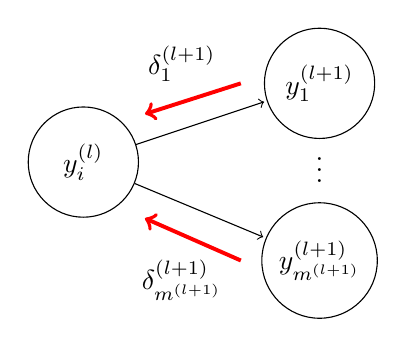
\begin{tikzpicture}[shorten >=1pt]
     \tikzstyle{unit}=[draw,shape=circle,minimum size =1.4cm]

     \node[unit](i) at (0,1){$y_i^{(l)}$};
     \node[unit](k1) at (3,2){$y_1^{(l+1)}$};
	\node at (3, 1){$\vdots$};
	\node[unit](km) at (3,-0.25){$y_{m^{(l+1)}}^{(l+1)}$};
	
	\node at (1.25,2.25){$\delta_1^{(l+1)}$};
	\node at (1.25,-0.5){$\delta_{m^{(l+1)}}^{(l+1)}$};

       	\draw[->] (i) -- (k1);
	\draw[->] (i) -- (km);
	
	\draw[->,red,line width=0.05cm] (2,-0.25) -- (0.75,0.3);
	\draw[->,red,line width=0.05cm] (2,2) -- (0.75,1.6);
\end{tikzpicture}
 
\end{document}

